% =====================================================================
% DC -- Depth Curves. Furnace Research, 2026-08-24.
%
% Per-layer sign-free AUROC maps of commit-time attention morphology.
% Registered protocol: PRE_REGISTRATION.md (grid A, discovery) and
% PRE_REGISTRATION_EXPANSION.md (grid B, held-out-model confirmation),
% both in commit-confluence/exploratory/depth-curve/.
%
% Compile with pdfLaTeX or tectonic. Figures live in dc-figures/.
% Self-contained: inline thebibliography (no .bib).
% Preamble mirrors the RPV/ACE drafts for portability.
%
% DISCIPLINE (binding, from the registrations):
%   * E5 = WEAKEN 8/12 against a frozen >=10/12 + family bars. Never rounded up.
%   * E6 = NOT TESTED (gate closed). Never reported as a result.
%   * Grid A = discovery, grid B = confirmation. Never pooled numerically.
%   * Whole lane is torch/Modal, non-byte-comparable with sealed MLX panels.
%   * 405B never ran and is outside every denominator.
%   * Claim-1 phrasing is "no rule established", never "non-law proven".
% =====================================================================

\documentclass[10pt, letterpaper]{article}

\usepackage[margin=1in]{geometry}
\usepackage[T1]{fontenc}
\usepackage{microtype}
\usepackage{lmodern}
\usepackage{amsmath, amssymb, amsthm}
\usepackage{booktabs}
\usepackage{graphicx}
\usepackage{xcolor}
\usepackage{natbib}
\usepackage[hidelinks]{hyperref}
\usepackage[capitalise]{cleveref}
\usepackage{caption}
\usepackage{enumitem}
\usepackage{authblk}
\usepackage{placeins}

\graphicspath{{dc-figures/}}
\setlength{\parskip}{0.4em}
\captionsetup{font=small, labelfont=bf}

\title{Cross-Sections of Commitment\\
\large Per-layer separation maps of attention morphology}
\author[ ]{Michael S.R. Kitti}
\affil[ ]{Furnace Research (independent) \quad \texttt{msrkittty@proton.me}}
\date{August 24, 2026}

\begin{document}
\maketitle

\begin{abstract}
Internal-state probes for hallucination detection are almost always read at a
fixed depth --- a layer chosen once, then held constant across models. That
choice is rarely measured, and the cost of getting it wrong is unknown. We ask
the question a deployer would ask: \emph{if I must pick one layer, does any rule
tell me which?} We answer it with registered per-layer sign-free AUROC curves of
a sealed inter-head-disagreement metric, computed over every decoder block of
$10$ instruction-tuned models spanning four families and $28$--$88$ blocks, on
two hallucination-adjacent benchmarks. The confirmation bars were specified
after the discovery grid was seen and frozen before any confirmation curve was
inspected. Discovery on $8$ cells and prospective held-out-model confirmation on
$12$ more give three results. First, \textbf{no placement rule was established}: peak location is
model- and task-dependent, and neither the frozen absolute nor the frozen
relative rule fired. Second, a sparse depth panel can \textbf{invert} a locus
conclusion --- a three-rung panel classified \texttt{Llama-3.3-70B} as a
readout-locus model, while its full curve carries a broad mid-stack band peaking
at $0.8975$ on block $48/80$, above the $0.8156$ in-sample winner of the $29$-cell
panel that the rungs produced. Third, a terminal-block give-back appears in every
evaluable held-out cell but one ($p_{\mathrm{grid}}=0.0005$, pooled dip CI
$[0.123, 0.201]$) yet scores $8/12$ against a frozen bar of $\geq 10/12$ plus
family guards, and is therefore reported as \textbf{WEAKEN} --- a strong,
nearly-universal regularity whose registered confirmation bar it did not clear.
The secondary cliff endpoint was gatekept behind that confirmation and is
\textbf{NOT TESTED}. Three cells produced no number at all, for two distinct
reasons --- an operational gate, and twice an instrument-domain boundary where
the sealed metric is undefined under total attention-sink collapse --- and,
separately, one fully evaluable cell is a genuine miss. For deployment
the corollary is narrow and practical: measure the layer on the target model,
because the registered tests established no rule that would let you transfer one.
\end{abstract}

\section{Introduction}
\label{sec:intro}

\textbf{Probes are read at a depth, and the depth is usually guessed.} Work that
detects hallucination, deception, or failure from a model's internal state must
choose where in the stack to look. In practice that choice is made once --- a
mid-stack layer, the last layer, a small sweep on one model --- and then carried
to other models as though it were a property of transformers rather than a
property of the one model it was tuned on. The literature is candid that
placement matters~\citep{apollo2025probes, ruan2026abort}, but the shape of the
underlying curve is rarely published, so the size of the risk is unmeasured.

\textbf{The gap.} A deployer choosing a probe layer has one question: is there a
rule? Concretely --- does separation live at a fixed absolute offset from the
end of the stack, or at a fixed fraction of depth, or nowhere transferable at
all? Answering it requires the whole curve, not a sample of it, and it requires
deciding what would count as an answer \emph{before} looking.

\textbf{What we built.} We compute a per-layer separation map: for every decoder
block of a model, the sign-free AUROC of a sealed commit-time attention
disagreement statistic against the hallucination label, plus a shuffled-label
envelope that says what that block's AUROC looks like when the labels carry no
information. The instrument is cheap --- one forward pass per row, no training,
no gradient --- and it is registered. Grid~A ($8$ cells) is \emph{discovery};
grid~B ($12$ cells from six held-out models in three registered families) is
\emph{prospective confirmation on two fixed benchmarks}, with every threshold, guard, and
denominator frozen in a pre-registration commit before extraction began, and a
scorer that runs exactly once.

\textbf{Contributions.}
\begin{enumerate}[leftmargin=1.4em, itemsep=0.15em]
  \item \textbf{A blind-spot result} (\cref{sec:blindspot}): a three-rung depth
    panel inverted a locus conclusion on a $70$B model. This bounds the
    interpretation of any fixed-layer probing claim, including our own prior
    panels, without changing their numbers.
  \item \textbf{A registered placement result} (\cref{sec:placement}): no
    transferable depth rule was established at this resolution. We state this as
    \emph{no rule established}, not as a proven non-law.
  \item \textbf{A registered regularity, reported as a miss}
    (\cref{sec:dip}): the terminal-block give-back is nearly universal and
    misses its own confirmation bar. We report the bar and the miss together.
  \item \textbf{Three failure modes, each a finding} (\cref{sec:failures}),
    including an instrument-domain boundary that every future use of the sealed
    metric must carry.
\end{enumerate}

\textbf{Scope, stated once and load-bearing.} Every cell in this paper is a
\texttt{torch}/Modal extraction. Eighteen of the twenty were specified
\texttt{nf4}; both task cells of \texttt{Mistral-Medium-3.5} use FP8-origin weights
deterministically dequantised for BF16 compute. None is byte-comparable with our
sealed MLX panels, and the two are never pooled. Grid~A rates are cited as discovery only and never enter a grid~B count.
Confirmation is claimed on two fixed benchmarks --- adversarial NLI
round~1~\citep{anli} and the QA split of HaluEval~\citep{halueval} --- and
nothing here is task-general. We make no causal,
lineage, or post-training claims, and no factorial family$\times$scale claim: the
comparative panel is unbalanced by construction.

\section{The instrument}
\label{sec:instrument}

\textbf{One forward pass per row, one number per block, and a null that says what
noise looks like.} For each input row we run the model to its commitment token
and read, at every decoder block $\ell \in \{0, \dots, N-1\}$, a sealed
attention-morphology statistic: the Jensen--Shannon disagreement among that
block's attention heads over the prompt, computed with the BOS position excluded
(\texttt{final\_js\_no\_bos}, our pre-registered primary). Three secondary
metrics are banked alongside it and are not analysed here. ``Block'' and
``decoder layer'' denote the same object throughout.

\paragraph{Sign-free AUROC.} Each cell contributes $200$ rows, exactly
$100$ hallucinated and $100$ faithful. For every block we compute
$A_\ell = \max\{\mathrm{AUROC}_\ell,\, 1-\mathrm{AUROC}_\ell\}$, which measures
separation without committing to a direction. This is deliberate and it is a
limitation we carry openly: sign-free AUROC is computed in-sample and cannot be
deployed as-is, because the sign must itself be fit. It is the right instrument
for the question \emph{where is there signal at all}, and the wrong one for
\emph{how well would a probe here perform}.

\paragraph{The envelope.} For each \emph{grid-A} cell we redraw the labels $200$
times under a fixed seed and record the $97.5$th percentile of the resulting
per-block sign-free AUROC. No envelope was registered for grid-B cells, and none
is shown for them anywhere in this paper. This envelope is the paper's honesty floor: because $A_\ell$ is
a maximum over two directions it is bounded below by $0.5$ and drifts upward with
finite samples, so a raw AUROC of $0.58$ can be pure noise. Only blocks above
their own envelope are treated as carrying signal. A \emph{qualifying peak}
$\ell^*$ is the block maximising $A_\ell$ subject to $A_\ell \geq 0.65$ and
$A_\ell > \mathrm{env}_\ell$; a cell with no such block is undefined, and
undefined counts as a failure in every registered denominator.

\paragraph{Two grids, and what separates them.} Grid~A ($4$ models $\times$ $2$
tasks) is \textbf{discovery}: it is where the dip and cliff regularities were
first seen, and its rates are cited as discovery throughout. Grid~B ($6$
held-out models $\times$ $2$ tasks $=12$ cells) is \textbf{prospective
held-out-model confirmation on two fixed benchmarks}. Grid~B endpoints are
measured with \emph{cross-fitted} estimators: rows are split into $K=5$ folds,
the peak is located on each training fold, and the endpoint is evaluated on the
held-out rows, which removes the selection bias that an in-sample argmax carries.
Before grid~B ran we re-scored grid~A under exactly these estimators, so the
discovery rates quoted for calibration ($8/8$ for the dip, $7/8$ for the cliff)
are measured with the same instrument as the confirmation.

\paragraph{What was frozen, and when.} The grid-B pre-registration commit pins
the endpoint definitions, the decision bars, the family guards, the denominator,
the model revisions, and the extraction and scoring code together. Smoke runs are
gates-only and never emit a per-block AUROC. The scorer runs \emph{once}, after
all twelve cells reach a terminal status. No grid-B threshold moved after the
freeze and no grid-B endpoint was scored twice. The grid-A re-score described
above is a distinct, pre-freeze calibration step and is always labelled as one.

\section{The blind spot}
\label{sec:blindspot}

\textbf{A three-rung depth panel classified a model's locus, and the full curve
says the classification was an artifact of where the rungs fell.} Our own prior
panels --- and, we suspect, a good deal of fixed-layer probing work --- sample
depth at three points: the middle block, the penultimate block, and the last
block ($\ell \in \{\lfloor N/2 \rfloor,\, N-2,\, N-1\}$). On
\texttt{Llama-3.3-70B-Instruct}/\texttt{anli\_r1} that panel found its best
attention cell weak and its best readout cell strong, and the family was recorded
as ``readout locus''.

\Cref{fig:money} shows what those three rungs were sampling. The full curve
carries a broad mid-stack band: $44$ of $80$ blocks sit above the shuffled
envelope, whose ceiling is $0.6145$, and the qualifying peak is $A_{48}=0.8975$.
The three rungs land at blocks $40$, $78$ and $79$. Two of them sit inside the
envelope --- statistically indistinguishable from shuffled labels --- and the
third clears it by about $0.02$. The band was not merely under-sampled; it
was missed on all three draws.

\paragraph{The comparison, stated carefully.} The panel's winner was a
\emph{readout} cell scoring $0.8156$ across a $29$-cell panel, and $0.8975 >
0.8156$. Three qualifications travel with that inequality and none of them may be
dropped. (i)~Both numbers are \emph{in-sample}: $0.8156$ is the panel's in-sample
full-panel marginal, quoted here for like-for-like comparison against an
in-sample depth curve. The same winner's deployed out-of-bag median is $0.7954$
with interval $[0.6995, 0.8728]$ and winner stability $0.511$, so a reader must
not take $0.8975$ as beating a bootstrapped bound. (ii)~The two quantities come
from \emph{different instruments}: a readout cell read at the commitment step is
not an attention-morphology cell read at a block, and \cref{fig:money} is
therefore a cross-instrument comparison. (iii)~$0.8156$ is the winner of the full
$29$-cell panel, not of its readout subset, so the accurate phrasing is that the
mid-stack peak exceeds \emph{the panel winner}.

\paragraph{What this does and does not license.} It does not change a single
panel number, and it does not falsify the panel's winner: on the rungs it
sampled, the panel reported correctly. What it bounds is \emph{interpretation}.
``This family reads out late'' was never measured; it was inferred from three
samples that happened to straddle a band. Any claim of the form ``family $F$
localises signal at region $R$'', ours included, inherits this caveat unless the
curve behind it was measured. The same model's \texttt{halueval\_qa} curve
carries a band that is broader and earlier still ($54/80$ blocks above envelope,
$\ell^*=26$), so this is not a single-cell accident.

\begin{figure}[t]
  \centering
  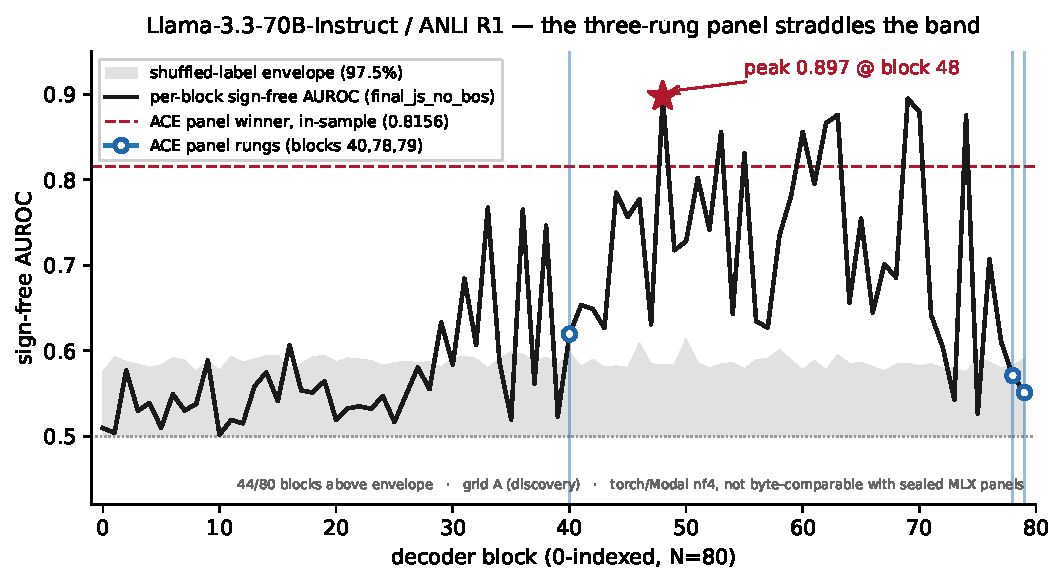
\includegraphics[width=\linewidth]{fig2_money_llama33_anli.pdf}
  \caption{\textbf{The blind spot.} Per-block sign-free AUROC for
  \texttt{Llama-3.3-70B-Instruct}/\texttt{anli\_r1} (grid~A, discovery). Shaded
  band is the $97.5$\% shuffled-label envelope. Circles mark the three rungs a
  fixed-depth panel samples ($40$, $78$, $79$ of $80$); two lie inside the
  envelope. The dashed line is the in-sample winner of that panel's full $29$ cells
  ($0.8156$, a readout cell read at the commitment step --- a different
  instrument, shown for scale, not as a matched baseline). Both numbers are
  in-sample: the same winner's deployed out-of-bag median is $0.7954$
  $[0.6995, 0.8728]$ with stability $0.511$, so the peak does not beat a
  bootstrapped bound.
  The qualifying peak is $0.8975$ at block $48$. Grid~A only; \texttt{torch}/Modal
  \texttt{nf4}, not byte-comparable with sealed MLX panels.}
  \label{fig:money}
\end{figure}

\section{The terminal give-back: a regularity that missed its bar}
\label{sec:dip}

\textbf{The primary endpoint scores $8/12$ against a frozen bar of $\geq 10/12$
plus family guards, and is therefore WEAKEN, not CONFIRM.} We state the miss
before the anatomy, because the anatomy is unusually favourable and would
otherwise read as a rescue.

\paragraph{What was registered.} E5 asks whether separation gives back at the
very end of the stack: whether the final block scores materially below the
qualifying peak. A cell succeeds when the cross-fitted dip magnitude
$\Delta_{cf} \geq 0.05$ with all five folds qualifying. The decision rule, frozen
before extraction: \textbf{CONFIRM} at $\geq 10/12$ successes \emph{and}
$\geq 3/4$ in each of the three grid-B families \emph{and} pooled
$p_{\mathrm{grid}} < 0.05$; \textbf{WEAKEN} at $8$--$9/12$, or $\geq 10/12$ with a
family or $p$ failure; \textbf{FALSIFY} at $\leq 7/12$. The denominator is always
$12$: missing, gate-aborted, and no-qualifying-peak cells count as failures.

\paragraph{What happened.} Eight of twelve. Families $4/2/2$ against a $\geq 3/4$
guard that two of three families miss. Pooled $p_{\mathrm{grid}} = 0.0005$. Two
of the three CONFIRM conditions therefore fail, and the registered decision is
\textbf{WEAKEN}.

\paragraph{The anatomy, labelled descriptive.} Of the nine evaluable cells, eight
show the dip; the pooled dip interval is $[0.123, 0.201]$; the registered
evaluable-only sensitivity recount is $8/9$ and the leave-Medium-out recount is
$6/10$. \Cref{fig:forest} shows every cell with its interval. This is the honest
summary: \emph{the terminal give-back appears in every evaluable held-out cell but
one, and the registered bar priced in exactly the failures that materialised.}
The frozen denominator counts the three aborted cells against the endpoint by
design, precisely so that an instrument that fails to produce a number cannot be
quietly excluded from its own test. We report it as written --- a strong,
nearly-universal regularity whose registered confirmation bar it did not clear.
Neither the $p$-value nor the $8/9$ sensitivity is a softer bar, and neither is
offered as one.

\paragraph{The one true miss.} \texttt{Mistral-Small-3.2-24B}/\texttt{halueval\_qa}
returns $\Delta_{cf}=0.0045$ --- not a failure of measurement but a cell where the
terminal give-back genuinely is not there. It sits essentially on zero in
\cref{fig:forest} and it is the reason the regularity is ``nearly'' universal
rather than universal.

\begin{figure}[t]
  \centering
  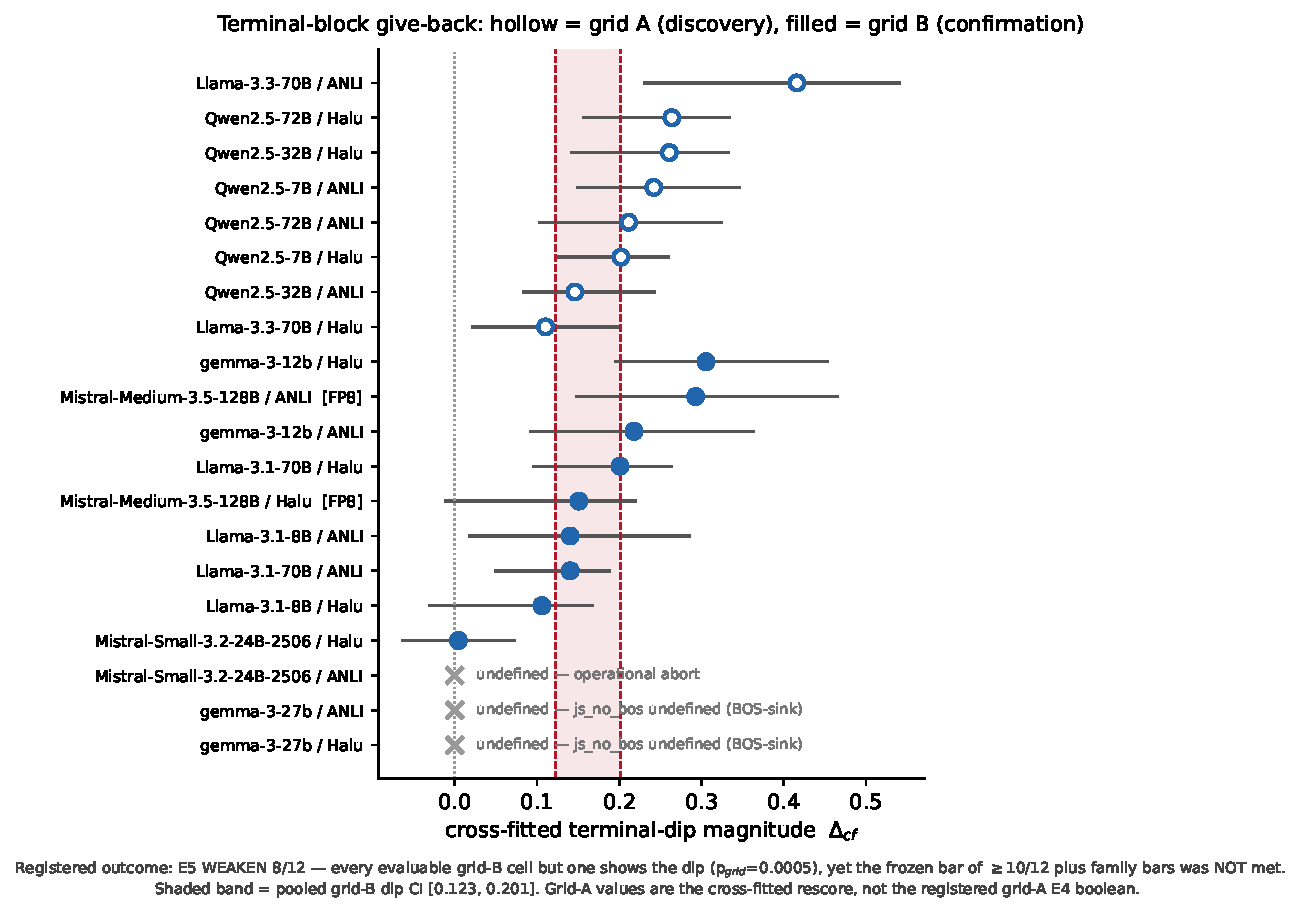
\includegraphics[width=0.92\linewidth]{fig3_terminal_dip_forest.pdf}
  \caption{\textbf{Terminal-block give-back, all cells.} Cross-fitted dip
  magnitude $\Delta_{cf}$ with $5$--$95$ intervals. Hollow markers are grid~A
  (discovery, re-scored under the grid-B estimators --- \emph{not} the registered
  grid-A boolean); filled markers are grid~B (confirmation). Shaded band is the
  pooled grid-B interval $[0.123, 0.201]$. The three undefined cells are shown
  with their reasons distinguished and are counted as failures in the $12$-cell
  denominator. \texttt{Mistral-Medium-3.5} is FP8-origin.}
  \label{fig:forest}
\end{figure}

\subsection*{The cliff endpoint was not tested}
\label{sec:cliff}

\textbf{E6 is NOT TESTED, and no cliff result is reported in this paper.} The
registration gatekeeps the cliff endpoint behind an E5 CONFIRM. E5 did not
CONFIRM, so the gate closed and no confirmatory cliff evaluation ever ran. This
is not a null result and it must not be read as one: a gatekept endpoint that was
never evaluated has no verdict at all.

What we may show is the grid-A discovery observation that motivated registering
it. \Cref{fig:cliff} plots, per grid-A cell, the largest single-block jump $J$
against the total rise $R$. In seven of eight discovery cells the rise arrives in
roughly one block. That is \emph{discovery only}; it carries no confirmatory
status, and the grid-B descriptive rate ($2/12$, depressed by early-peak cells
that the registration defines as cliff-undefined) is reported without
interpretation. One grid-A cell is excluded from \cref{fig:cliff} entirely:
\texttt{Llama-3.3-70B}/\texttt{halueval\_qa} reports $J=0.0000$, but that zero is
a structural empty-window fallback --- its peak at block $26$ falls below the
jump-search floor, leaving the search segment empty --- and plotting it as a
measured absence of a jump would be a fabrication.

\begin{figure}[t]
  \centering
  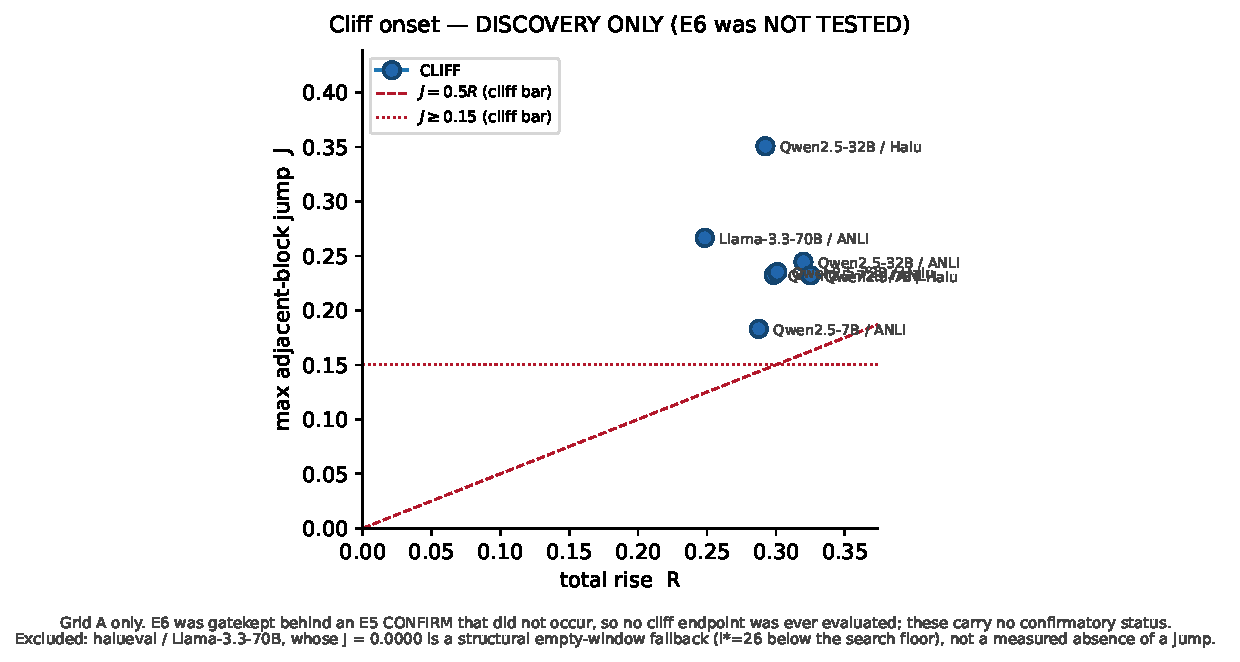
\includegraphics[width=0.62\linewidth]{fig5_cliff_onset.pdf}
  \caption{\textbf{Cliff onset --- DISCOVERY ONLY.} Grid~A cells: largest
  adjacent-block jump $J$ against total rise $R$, with the two registered cliff
  bars drawn. E6 was gatekept behind an E5 CONFIRM that did not occur, so no
  cliff endpoint was ever evaluated and these points carry no confirmatory
  status. \texttt{Llama-3.3-70B}/\texttt{halueval\_qa} is excluded: its
  $J=0.0000$ is a structural empty-window fallback, not a measured zero.}
  \label{fig:cliff}
\end{figure}

\section{Placement: no rule established}
\label{sec:placement}

\textbf{Neither frozen placement rule fired, and the descriptive panel beside
them tests no law at all.} Grid~A registered two candidate
rules and a tie-breaker between them. An \emph{absolute} rule --- separation
peaks a fixed number of blocks from the end --- required the spread of $N-\ell^*$
to be at most $2$ blocks. A \emph{relative} rule --- separation peaks at a fixed
fraction of depth --- required the spread of $\ell^*/N$ to be at most $0.015$.
Neither came close, and the registered outcome is \textbf{UNDECIDED}: at this
resolution, \emph{no placement rule was established}. Note the scope precisely ---
E1 is a \emph{grid-A} endpoint, so the frozen rules were tested on four discovery
models, not on all ten. The ten-model panel below is registered as descriptive and
is explicitly forbidden from making law or non-law claims. We phrase it that way
deliberately. Failing to establish a rule --- on four discovery models at $n=200$
per cell, with a ten-model descriptive panel that offers no obvious replacement ---
is not the same as proving no rule exists, and this paper does not claim the
stronger thing.

\paragraph{An artifact that looked like a law.} Before the full curves existed, a
three-rung panel appeared to show separation peaking at $N-2$. It does not, and
the reason is the sampling failure \cref{sec:blindspot} documents in its other
guise: $N-2$ merely won among three sampled points. On the full curves the six
\texttt{Qwen2.5} peaks are spread from $N-2$ to $N-17$, at depth fractions $0.79$
to $0.93$ --- one of them does land at $N-2$, but a spread of $15$ blocks is far
too wide for the frozen absolute rule, and a fraction range that broad is far too
wide for the relative one.

\paragraph{The panel.} \Cref{fig:peakfrac} plots cross-fitted peak fraction
against depth for all $17$ evaluable cells. Grid~A and grid~B are drawn
separately and are never pooled numerically. There are no confidence intervals on
these points, and their absence is deliberate: no bootstrap interval for this
estimator is banked on either grid, and grid~A's peak-location interval belongs
to a \emph{different} estimator (the in-sample argmax), so splicing it onto
cross-fitted points would silently mix two things. We plot instead the spread of
the five cross-fitted training-fold peaks, which is what we actually have.

\begin{figure}[t]
  \centering
  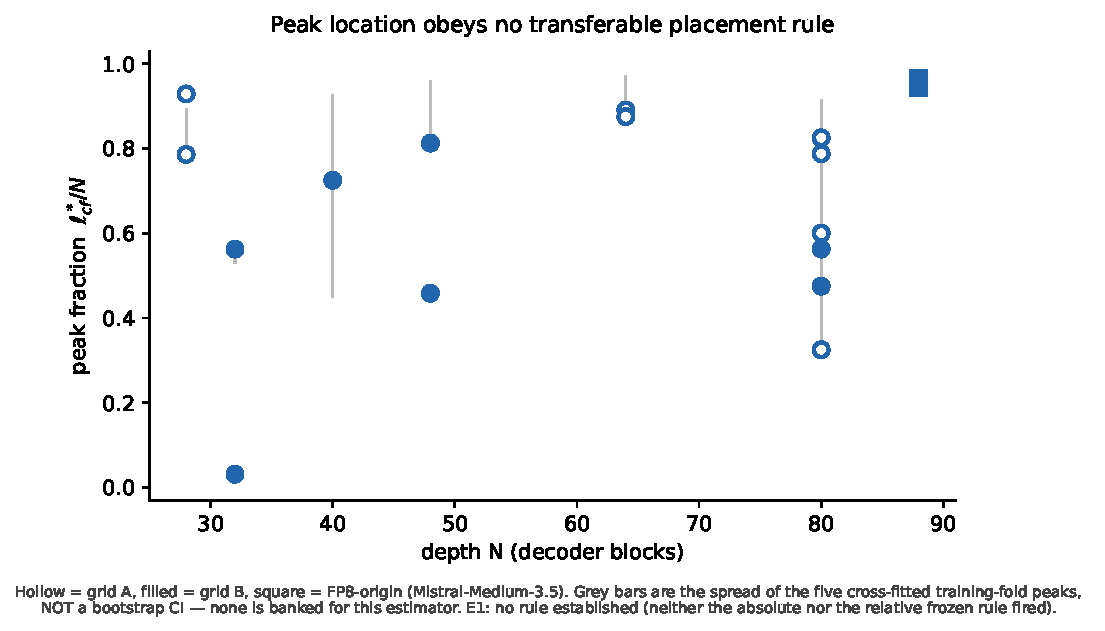
\includegraphics[width=0.88\linewidth]{fig4_peak_fraction.pdf}
  \caption{\textbf{No placement rule established.} Cross-fitted peak fraction
  $\ell^*_{cf}/N$ against depth $N$. Hollow = grid~A, filled = grid~B, square =
  FP8-origin. Grey bars are the spread of the five cross-fitted training-fold
  peaks, \emph{not} a bootstrap interval --- none is banked for this estimator.
  Grid~A and grid~B are shown together for visual context only and are never
  pooled numerically.}
  \label{fig:peakfrac}
\end{figure}

\paragraph{Family structure, descriptive only.} Mean peak fractions cluster by
family: \texttt{Mistral} $0.88$ and \texttt{Qwen} $0.85$ peak late,
\texttt{Llama-3.1} $0.41$ and \texttt{Llama-3.3} $0.46$ peak mid, \texttt{Gemma}
$0.64$ falls between. This is structure, and it is not a rule --- with two models
per family, family is fully confounded with tokenizer, architecture, and size,
and we make no factorial claim. Two registered descriptive predictions about the
Llama band were both borne out \emph{on \texttt{anli\_r1}}, the only task over
which they were registered: the qualifying-block count in the mid region was
$\geq 10$ in a majority of folds for \texttt{Llama-3.1-70B}, and $<5$ in a majority
for \texttt{Llama-3.1-8B}. The registration
forbids ``replicates'', ``stable'' and ``emergent'' vocabulary here and we honour
that: this is a same-size version comparison in which base-checkpoint identity
was never established.

\section{Three failure modes, three findings}
\label{sec:failures}

\textbf{Three of twelve grid-B cells produced no number, and the three reasons
are scientifically distinct.} They count identically against the endpoint --- all
three are failures in the frozen denominator --- but conflating them in the
discussion would hide the most transferable result in this paper.

\paragraph{A behavioral gate (operational).}
\texttt{Mistral-Small-3.2-24B}/\texttt{anli\_r1} never produced a curve: the
extraction aborted on a missing prompt manifest. This is an operational failure
with no bearing on the instrument, and we record it as one. It counts as a
failure because the registration says every non-producing cell does.

\paragraph{An instrument-domain boundary (the transferable one).} Both
\texttt{gemma-3-27b-it} cells aborted with the sealed primary metric returning
\emph{undefined} at block~$3$, row~$0$. The cause is not a bug: under a total
attention-sink collapse, essentially all attention mass concentrates on the BOS
position, and a statistic defined on the non-BOS distribution has no distribution
left to measure. \texttt{final\_js\_no\_bos} therefore has a \emph{domain}, and
\texttt{gemma-3-27b} sits outside it.

This is a standing caveat for every future use of the metric, in this paper and
elsewhere: where the sink collapses, the value must be rendered and reported as
explicitly undefined --- never as zero, and never silently dropped. A zero would
read as ``the heads agree completely'', which is the opposite of what the model
is doing; a dropped cell would quietly shrink a denominator. Both figures and
tables in this paper mark these cells undefined for exactly this reason.

\paragraph{One true miss (the honest one).} The third is not a failure of the
apparatus at all: \texttt{Mistral-Small-3.2-24B}/\texttt{halueval\_qa} produced a
clean curve whose terminal dip is $\Delta_{cf}=0.0045$. The regularity is simply
absent there. A registered endpoint that never encounters a genuine miss has not
been tested very hard.

\section{The full picture}
\label{sec:grid}

\Cref{fig:grid} shows every curve in the study. \Cref{tab:cells} gives the
per-cell numbers and \cref{tab:ledger} gives every registered endpoint beside its
frozen bar and its actual outcome. Two reading instructions travel with them.
First, grid~A panels carry their registered shuffled envelope and grid~B panels
do not: no envelope was ever registered for grid-B slugs, and computing one after
the verdict would be a new Monte-Carlo statistic on confirmatory cells. Grid-B
curves are recomputed from the banked extractions through the registered scorer's
own validating loader --- which re-checks the frozen data hash, the pinned model
revision, and both extraction gates --- but they are shown unshaded, and their
absence of shading is a statement about the registration, not about the data.
These recomputed curves are \textbf{post-verdict descriptive rendering and carry no
confirmatory status}: the registered grid-B scorer banked no per-block curve, and
nothing in \cref{sec:dip} or \cref{sec:placement} depends on them.
Second, several columns of \cref{tab:cells} are empty for grid~B. They are marked
\texttt{--}, meaning \emph{not scored for that grid}, not \emph{missing}:
peak AUROC, mid-region median, rise-shape and peak-location interval were never
computed for grid~B, and backfilling any of them now would be new computation on
confirmatory cells.

\begin{figure}[p]
  \centering
  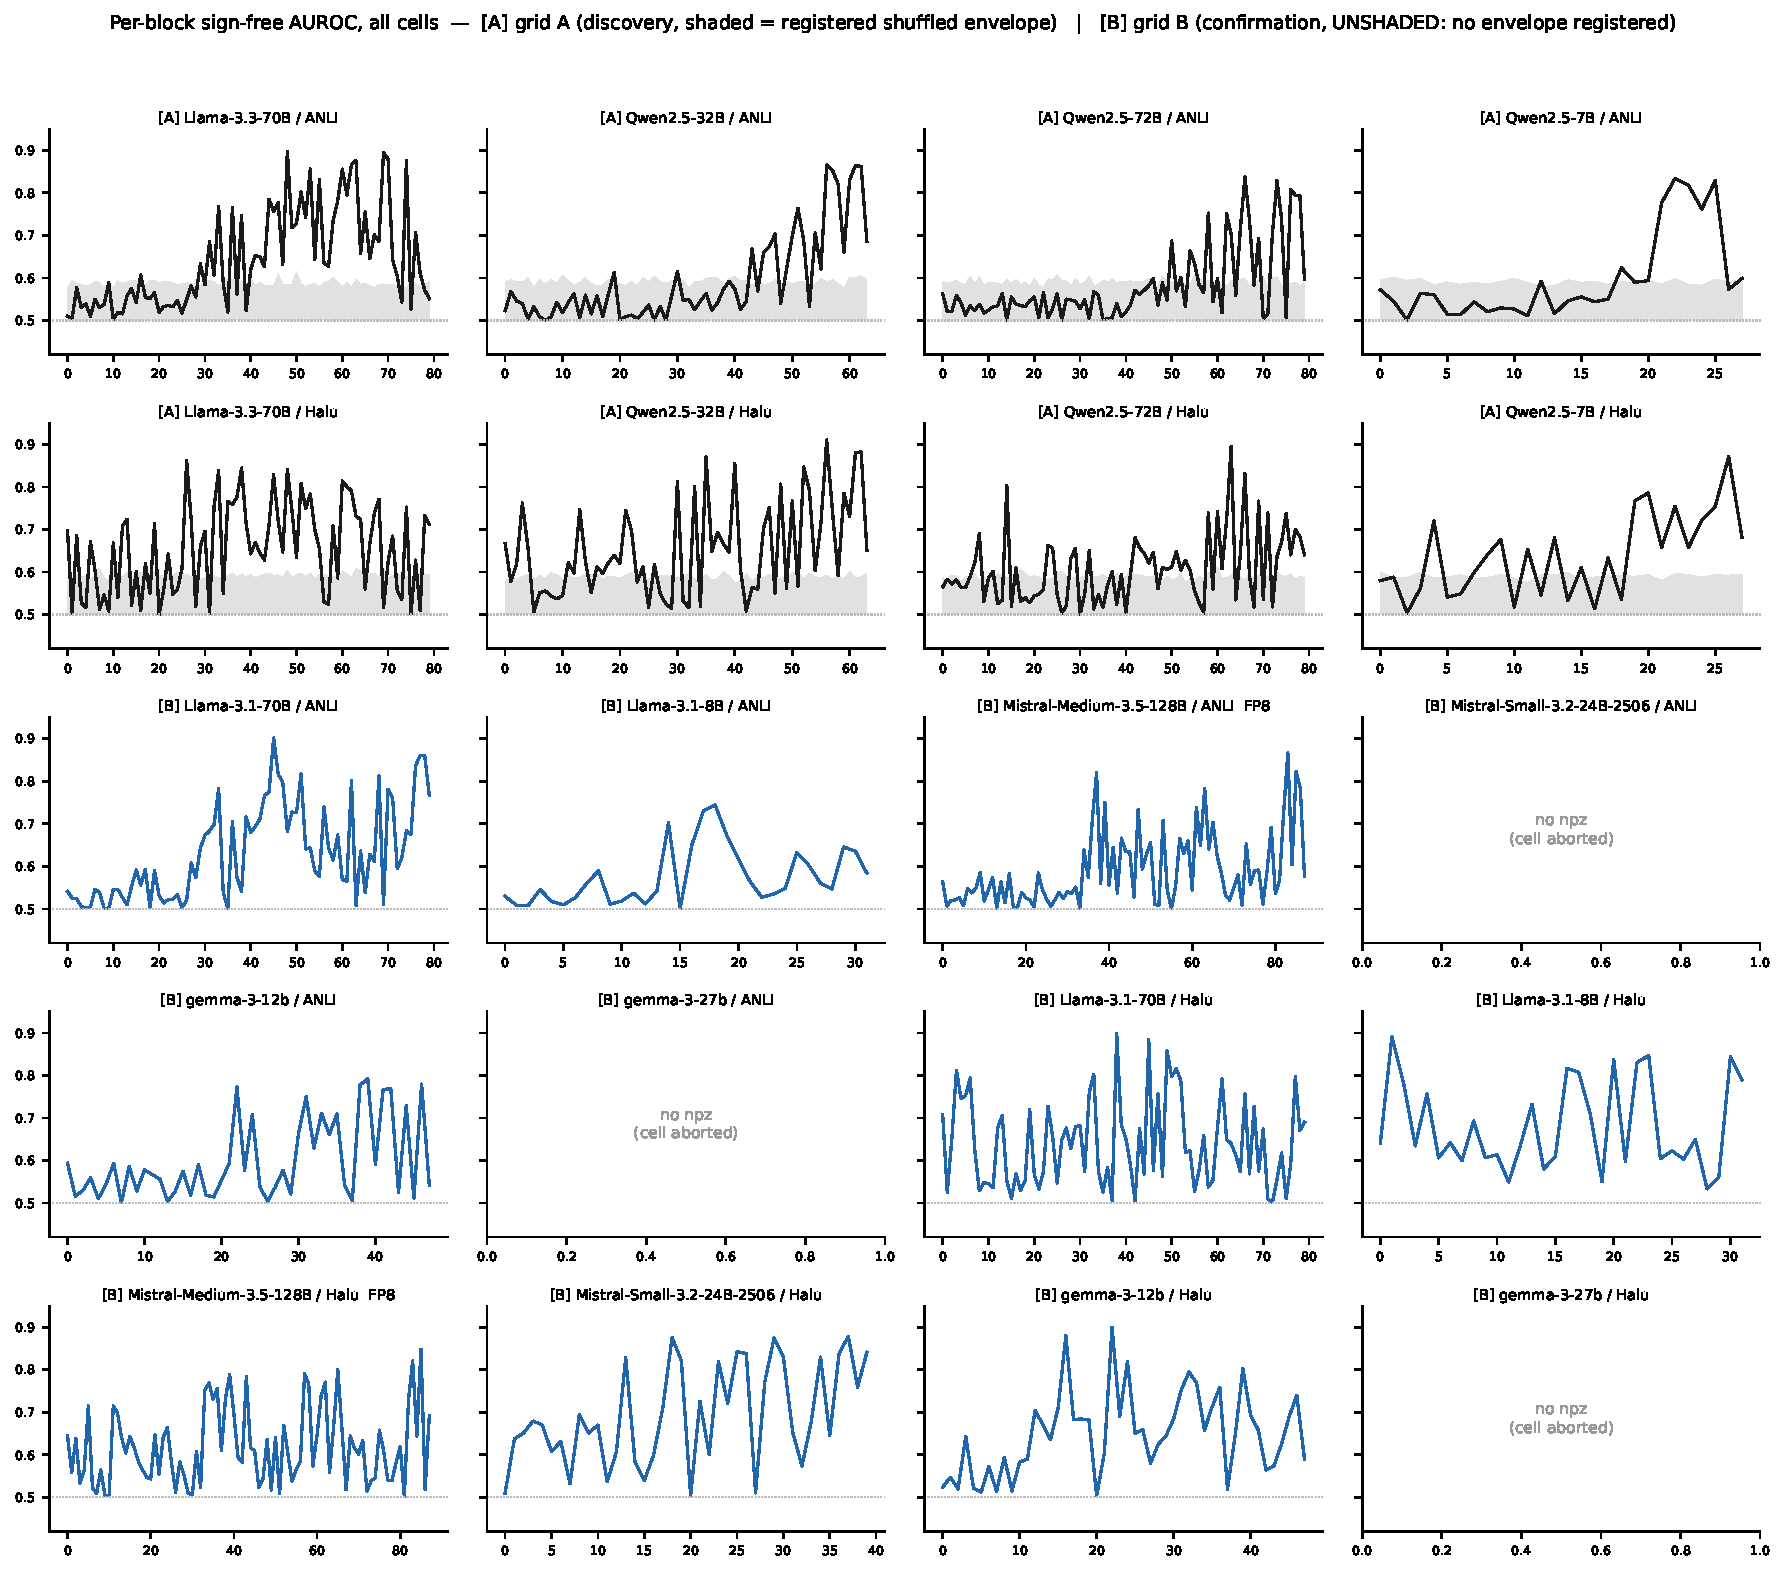
\includegraphics[width=\linewidth]{fig1_depth_curve_grid.pdf}
  \caption{\textbf{Every depth curve in the study.} Per-block sign-free AUROC.
  Top block, black: grid~A (discovery), shaded with its registered $97.5$\%
  shuffled-label envelope. Lower block, blue: the grid-B \emph{cells}, drawn from
  curves recomputed after the single-look scoring --- these curves are post-verdict
  descriptive rendering and carry no confirmatory status, and they are deliberately
  unshaded because no envelope was registered for grid-B cells. Three grid-B cells
  produced no extraction and are shown as labelled empty panels rather than
  omitted. The two grids are never pooled numerically.}
  \label{fig:grid}
\end{figure}

\begin{table}[t]
  \centering\footnotesize
  \begin{tabular}{llrrlllll}
\toprule
cell & grid & N & peak blk & peak CI & peak AUROC & mid med & E2 & $\Delta_{cf}$ \\
\midrule
Llama-3.3-70B / ANLI & A & 80 & 48 & [48, 74] & 0.8975 & 0.649 & CLIFF & 0.4160 \\
Qwen2.5-32B / ANLI & A & 64 & 56 & [56, 62] & 0.8655 & 0.545 & CLIFF & 0.1460 \\
Qwen2.5-72B / ANLI & A & 80 & 66 & [66, 77] & 0.8376 & 0.539 & CLIFF & 0.2115 \\
Qwen2.5-7B / ANLI & A & 28 & 22 & [22, 25] & 0.8336 & 0.546 & CLIFF & 0.2420 \\
Llama-3.3-70B / Halu & A & 80 & 26 & [26, 48] & 0.8621 & 0.721 & GRADUAL & 0.1105 \\
Qwen2.5-32B / Halu & A & 64 & 56 & [35, 61] & 0.9106 & 0.618 & CLIFF & 0.2610 \\
Qwen2.5-72B / Halu & A & 80 & 63 & [63, 63] & 0.8961 & 0.595 & CLIFF & 0.2640 \\
Qwen2.5-7B / Halu & A & 28 & 26 & [26, 26] & 0.8713 & 0.546 & CLIFF & 0.2020 \\
Llama-3.1-70B / ANLI & B & 80 & 45 & -- & -- & -- & -- & 0.1405 \\
Llama-3.1-8B / ANLI & B & 32 & 18 & -- & -- & -- & -- & 0.1405 \\
Mistral-Medium-3.5-128B / ANLI & B & 88 & 83 & -- & -- & -- & -- & 0.2930 \\
Mistral-Small-3.2-24B-2506 / ANLI & B & 40 & -- & -- & -- & -- & -- & undef. \\
gemma-3-12b / ANLI & B & 48 & 39 & -- & -- & -- & -- & 0.2180 \\
gemma-3-27b / ANLI & B & 62 & -- & -- & -- & -- & -- & undef. \\
Llama-3.1-70B / Halu & B & 80 & 38 & -- & -- & -- & -- & 0.2010 \\
Llama-3.1-8B / Halu & B & 32 & 1 & -- & -- & -- & -- & 0.1060 \\
Mistral-Medium-3.5-128B / Halu & B & 88 & 85 & -- & -- & -- & -- & 0.1510 \\
Mistral-Small-3.2-24B-2506 / Halu & B & 40 & 29 & -- & -- & -- & -- & 0.0045 \\
gemma-3-12b / Halu & B & 48 & 22 & -- & -- & -- & -- & 0.3055 \\
gemma-3-27b / Halu & B & 62 & -- & -- & -- & -- & -- & undef. \\
\bottomrule
\end{tabular}
% NOTE: '--' in grid-B rows means NOT SCORED for grid B, not missing data.
% Grid A peak blk = in-sample lstar; grid B peak blk = cross-fitted peak_cf (different estimator).
% Delta_cf for grid A is the cross-fitted rescore, NOT the registered grid-A E4 boolean.
% Mistral-Medium-3.5 is FP8-origin (dequantised to bf16).

  \caption{\textbf{Per-cell verdict table.} \texttt{--} means \emph{not scored for
  that grid}, not missing data. Grid-A peak block is the in-sample $\ell^*$;
  grid-B peak block is the cross-fitted $\ell^*_{cf}$ --- a different estimator,
  never compared numerically across the two. $\Delta_{cf}$ for grid~A is the
  cross-fitted re-score, not the registered grid-A boolean.
  \texttt{Mistral-Medium-3.5} is FP8-origin.}
  \label{tab:cells}
\end{table}

\begin{table}[t]
  \centering\footnotesize
  \begin{tabular}{llp{5.2cm}p{4.2cm}p{4.4cm}}
\toprule
id & endpoint & frozen bar & actual & outcome \\
\midrule
E5 & terminal-block give-back & CONFIRM if $\geq$10/12 AND $\geq$3/4 in each of 3 families AND $p_{grid}<0.05$; WEAKEN if 8--9/12; FALSIFY if $\leq$7/12 & 8/12; families 4/2/2; $p_{grid}$=0.0005 & WEAKEN -- count and family bars both missed \\
E6 & cliff onset & gatekept on E5 == CONFIRM; then $\geq$9/12 AND $\geq$4/6 per task AND $\geq$2/4 per family AND $p_{grid}<0.05$ & gate closed (E5 did not CONFIRM); descriptive-only count 2/12 carries no verdict & NOT TESTED -- no cliff endpoint was ever evaluated \\
E7 & cross-task peak distance & descriptive-registered, no bar, no verdict vocabulary & 6 models reported & descriptive \\
E8 & Llama mid-stack band context & descriptive-registered, no bar & P8 hit on ANLI ($\geq$10 qualifying mid-blocks, majority of folds, 3.1-70B); P9 hit on ANLI ($<$5, 3.1-8B) & descriptive \\
E1'' & peak-fraction panel & descriptive-registered, no bar & no transferable placement rule fired & descriptive -- no rule established \\
\bottomrule
\end{tabular}
% Denominator is ALWAYS 12, including the 3 aborted cells.
% Sensitivity (registered): leave-Medium-out E5 6; evaluable-only E5 8/9.
% Reported as written: a registered miss is a miss.

  \caption{\textbf{Registered endpoint ledger.} Every endpoint with its frozen bar
  and its actual outcome. The denominator is always $12$, including the three
  aborted cells.}
  \label{tab:ledger}
\end{table}

\FloatBarrier

\section{Related work: who measures the layer, and who assumes it}
\label{sec:related}

\textbf{Six recent internal-state detectors span the full range from measuring the probe layer
to assuming it, and the assumption is the more common practice.} We group them on that axis
because it is the axis this paper is about. Four study \emph{deception} and two
hallucination; five read the residual stream rather than attention morphology, so none is a
replication of anything here; they are convergent evidence about \emph{depth}.

\paragraph{Measured, and closest to what we plot.} \citet{dombrowski2024lying} trace
information-theoretic quantities --- predicted-token probability, entropy, and KL divergence to
the final layer --- through \emph{every} layer via the logit lens, on a Mistral-lineage 7B and two
Llama-2 chat models, read at the token immediately \emph{before} the model commits to a true or
false completion. That is the object shape of \cref{fig:money}: a per-layer curve of a scalar,
compared across a binary condition, at the commitment position. Two findings bear on ours.
On their stronger datasets separation opens mid-stack, around layers $15$--$20$ of $32$, not at the
terminal block. And its strength is \emph{dataset-dependent}: on \texttt{FreebaseStatements} the
truth and lie conditions only separate at layer $28$, which they attribute to the model being less
certain of the truth in that context. A
placement rule would have to survive that dependence, and \cref{sec:placement} reports that ours
did not. They also note that earlier probing work reads hidden states \emph{after} the statement
is produced --- an independent statement of the commit-locus position measured here. Their
instrument is the unembedded predictive distribution and ours is attention morphology, so the
correspondence holds at the level of depth phenomenology only.

\paragraph{Measured, and deployed.} \citet{apollo2025probes} fit a deception probe in the
\texttt{Llama-3.3-70B} residual stream at layer $22$ of $80$, chosen by sweep; their appendix
shows the usable deployment band is mid-stack and narrow, with recall at a fixed low
false-positive rate collapsing within a couple of layers while AUROC stays respectable.
\citet{ruan2026abort} make the sweep part of the method: probe layer is fixed \emph{per model} by
a preliminary per-layer AUC sweep, landing at $14/28$ for a $3$B Llama and $20/28$ for a $7$B
Qwen. That is \cref{sec:deployment}'s corollary already in production.

\paragraph{Measured, and dependent on the target as well as the model.}
\citet{kossen2024sep} fit linear probes on the residual stream to predict binarised semantic
entropy from a single generation, and report per-layer AUROC across five models, four
question-answering tasks and two token positions --- the broadest published depth panel we are
aware of, and one of the two papers here concerned with hallucination rather than deception. Two
things in it sharpen \cref{sec:deployment}. First, the band they select moves with the
\emph{supervision target}, not only with the model: on \texttt{Llama-3-70B}, fitting the same
architecture on the same data, the semantic-entropy probe is read at layers $76$--$80$ of $80$
while the accuracy probe is read at $31$--$35$, and on \texttt{Mistral-7B} the two bands are
$28$--$32$ and $12$--$16$ of $32$. Depth placement is therefore a property of the
(model, distribution, target) triple, which is a stronger requirement than the per-model sweep
of the preceding paragraph. Second, their bands are chosen by best mean AUROC
\emph{in-distribution and in-sample}, with no out-of-bag correction, and their
in-distribution verdict on which probe wins differs between the selected high-performing layers
and the layer range as a whole --- a reminder that the aggregation set is itself a degree of
freedom. It is the reason our registered endpoints are cross-fitted and why
\cref{sec:placement} reports argmax bands rather than argmax points. We claim no more than
that: the descriptive grid-A curves and their in-sample peaks --- including the $0.8975$
of \cref{sec:blindspot} --- are \emph{not} cross-fitted, and are labelled in-sample wherever
they appear. They additionally observe
that in their long-form setting AUROC more often peaks at intermediate rather than terminal
layers, attributing it to late layers being occupied with the next token; we record this as
phenomenology and do not treat it as evidence bearing on \cref{sec:dip}, since it is reported
without a dip statistic or interval, on a different instrument and a supervised target.

\paragraph{Measured on the step axis, and coarsely sampled on the layer axis.}
\citet{yeom2026commitment} vary \emph{position} where the four papers above vary depth. Aligning
generation trajectories on the step at which an answer concept is emitted, they report that the
correctness-predictive information in the output distribution is localised to that step: detection
AUROC is at chance two or more steps earlier, rises to $0.58$ at the emission step, and decays to
chance within a few steps after, while plain generated-token probability is flat across the same
window. The effect is modest in magnitude and clear in shape. Two things follow for us. It is
independent support for reading at the commitment position rather than aggregating over a
generation --- the locus this paper's instrument is measured at --- and it comes with the warning
that token entropy is a poor \emph{localiser} of that step, matching it in only $20\%$ of their
long-form trajectories. Their layer evidence points the other way, and we flag it as a caution
rather than a convergence. Their multi-layer probe table samples \emph{four} rungs --- first, middle,
last$-1$, last --- across four sizes of one family, and the winning rung is not stable across them:
middle for the $2$B and $4$B models, last$-1$ for the $0.8$B and $9$B. The mid-stack feature they
describe is the \emph{gap} between instruction-tuned and base models, not the probe AUROC itself,
which is a claim about what instruction tuning amplifies rather than about where a detector should
be read. A four-rung panel cannot separate those, which is the same limitation \cref{sec:placement}
reports for our own three-rung readout. We therefore take nothing from it about placement, and in
particular, as with \citet{kossen2024sep} above, we do not treat it as evidence bearing on
\cref{sec:dip} --- no dip statistic is reported, and \cref{sec:dip} is a registered miss whose
phrasing an external observation cannot alter.

\paragraph{Assumed.} \citet{hollinsworth2026solid} scale a lie-detector-gated oversight protocol
across Llama-3 models to $405$B parameters and Qwen-3 models to $32$B, and report a genuine
scaling trend: undetected deception falls from $34\%$ to $14\%$ at a fixed $99\%$ detector
true-positive rate. Their probe is read at $\lfloor L/2 \rfloor$ --- a fixed depth fraction applied
across two families spanning under a billion to $405$ billion parameters. We find no layer
ablation and no AUC-versus-layer curve reported in that paper. We flag this precisely, because it is the kind of choice this
paper is about and not a claim we can refute: absent a sweep there is no number to check
$\lfloor L/2 \rfloor$ against. What our results supply is a testable prediction. Our registered
peak fractions cluster by family (\cref{fig:peakfrac}), with the \texttt{Qwen} cells late in the
stack --- mean fraction $0.85$ --- and the Llama cells mid-stack. If detector accuracy were ever
plotted against layer at fixed model size in that setting, a mid-stack read should cost more for
Qwen-3 than for Llama-3. That is a prediction about a different construct on a different object,
offered as such.

Across the group: where placement is measured it is reported as model-specific --- and, in the one
case that varies the supervision target, target-specific too --- with a narrow usable band; where
it is assumed, it is assumed to be a constant fraction of depth. None of the
six reports a sweep supporting that constant. \Cref{sec:placement} is the nearest test of the
constant-fraction idea we are aware of --- on a different construct and a different object, and
neither frozen rule fired.

\section{What this means for probe placement}
\label{sec:deployment}

\textbf{Measure the layer; do not inherit it.} The deployment corollary is
narrow, and it is the practical point of the paper. If the registered absolute and
relative rules were both left unestablished on the discovery grid, and the
descriptive ten-model panel offers no obvious replacement, then a probe layer
imported from another model --- or from another size in the same family --- is an
untested assumption. The
replacement is cheap: one per-layer sweep on the target model, on a few hundred
labelled rows, costs a single forward pass per row and produces exactly
\cref{fig:money} for that deployment. \Cref{sec:related} shows this is already deployed
practice wherever anyone has looked: \citet{ruan2026abort} fix the probe layer per model by
exactly such a sweep, and one of their two models, \texttt{Qwen2.5-7B}, is in our own panel,
where the peak is likewise late.

The cost of not measuring is documented next door. \citet{apollo2025probes} find the usable band
mid-stack and narrow, with recall at a fixed low false-positive rate collapsing within a couple of
layers while AUROC stays respectable --- the same failure mode we report from the other side: an
aggregate score can look healthy at a layer where the deployable operating point has already
gone.

\section{Limitations}
\label{sec:limits}

\textbf{The honest list, and it is long enough to matter.}
\begin{itemize}[leftmargin=1.4em, itemsep=0.2em]
  \item \textbf{Sign-free and in-sample.} $A_\ell$ maximises over both directions
    and is computed in-sample. It answers \emph{where is there signal}, not
    \emph{how well would a probe do}. No number here is a deployment estimate.
  \item \textbf{$n=200$ per cell}, $100/100$. Peak locations are noisy at this
    resolution; the failure to establish a placement rule is a statement at
    \emph{this} resolution and a denser study could find one.
  \item \textbf{Two benchmarks.} Confirmation is claimed on \texttt{anli\_r1} and
    \texttt{halueval\_qa} and is not task-general.
  \item \textbf{Unbalanced panel.} Between one and three evaluable models per
    family, family confounded with tokenizer, architecture and size. No factorial claim; the version comparison
    establishes no base-checkpoint identity.
  \item \textbf{One precision-heterogeneous model, two cells.}
    \texttt{Mistral-Medium-3.5} contributes both of its task cells from FP8-origin
    weights, deterministically dequantised to BF16, and is flagged wherever it
    appears; the registered leave-Medium-out sensitivity is reported alongside the
    verdict.
  \item \textbf{Non-byte-comparable throughout.} All cells are \texttt{torch}/Modal
    and are never pooled with sealed MLX panels.
  \item \textbf{Per-cell argmax.} Peak selection is a maximum over $N$ blocks. The
    envelope and the cross-fitting mitigate the resulting optimism; they do not
    eliminate it.
  \item \textbf{Non-random evaluability.} Only $9$ of $12$ grid-B cells produced a
    number, and the three that did not are not a random sample: two are the same model
    failing the same instrument boundary. The endpoint counts them as failures, which
    is conservative, but the surviving nine are not an unbiased draw.
  \item \textbf{E1's frozen test covered four models.} The absolute and relative
    placement rules were grid-A endpoints. The ten-model panel is descriptive and
    tests no rule.
  \item \textbf{Grid-B full curves are post-verdict.} They were recomputed for
    \cref{fig:grid} after the single-look scoring and carry no confirmatory status;
    no endpoint depends on them.
  \item \textbf{No mechanism.} We report where separation lives, not why. Nothing
    here identifies a computation.
  \item \textbf{A frontier-scale cell was planned and never run.} A
    $405$B extraction was registered as a descriptive stretch, sat outside every
    confirmatory denominator by construction, and was not executed. No number in
    this paper depends on it.
\end{itemize}

\section*{Reproducibility}
Pre-registrations, extraction and scoring code, the banked per-cell arrays, and
the figure builder --- which asserts every plotted value against the scored
artifacts before writing a file --- are in the project repository at
\url{https://github.com/flowstyleliving/commit-confluence}, under
\texttt{exploratory/depth-curve/}.

\begin{thebibliography}{9}\footnotesize

\bibitem[Goldowsky-Dill et al.(2025)]{apollo2025probes}
N.~Goldowsky-Dill, B.~Chughtai, S.~Heimersheim, and M.~Hobbhahn.
\newblock Detecting strategic deception using linear probes.
\newblock \emph{arXiv:2502.03407}, 2025.

\bibitem[Ruan et al.(2026)]{ruan2026abort}
J.~Ruan, L.~Huang, Y.~Zhou, X.~Wei, H.~Wang, and M.~Sun.
\newblock Doomed from the start: Early abort of LLM agent episodes via a
  recall-controlled probe cascade.
\newblock \emph{arXiv:2607.06503}, 2026.

\bibitem[Kossen et al.(2024)]{kossen2024sep}
J.~Kossen, J.~Han, M.~Razzak, L.~Schut, S.~Malik, and Y.~Gal.
\newblock Semantic entropy probes: Robust and cheap hallucination detection in
  LLMs.
\newblock \emph{arXiv:2406.15927}, 2024.

\bibitem[Dombrowski \& Corlouer(2024)]{dombrowski2024lying}
A.-K. Dombrowski and G. Corlouer.
\newblock An information-theoretic study of lying in LLMs.
\newblock In \emph{Proceedings of the 41st International Conference on Machine
  Learning (ICML)}, PMLR 235, 2024.

\bibitem[Hollinsworth et al.(2026)]{hollinsworth2026solid}
O.~J. Hollinsworth, A.-K. Dombrowski, S.~Adam-Day, A.~Gleave, and C.~Cundy.
\newblock Scaling trends for lie detector oversight in preference learning.
\newblock In \emph{Proceedings of the 43rd International Conference on Machine
  Learning (ICML)}, PMLR 306, 2026. arXiv:2607.01567.

\bibitem[Yeom et al.(2026)]{yeom2026commitment}
J.~Yeom, J.~Sok, H.~Kim, S.~Park, J.~Park, and T.~Kim.
\newblock Hallucination as commitment failure: Larger LLMs misfire despite
  knowing the answer.
\newblock \emph{arXiv:2605.22007}, 2026.

\bibitem[Nie et al.(2020)]{anli}
Y.~Nie, A.~Williams, E.~Dinan, M.~Bansal, J.~Weston, and D.~Kiela.
\newblock Adversarial NLI: A new benchmark for natural language understanding.
\newblock In \emph{ACL}, 2020.

\bibitem[Li et al.(2023)]{halueval}
J.~Li, X.~Cheng, W.~X. Zhao, J.-Y. Nie, and J.-R. Wen.
\newblock HaluEval: A large-scale hallucination evaluation benchmark for large
  language models.
\newblock In \emph{EMNLP}, 2023.

\end{thebibliography}

\end{document}
